\documentclass[11pt, a4paper]{article}

% --- Packages ---
\usepackage[margin=0.9in]{geometry}
\usepackage[T1]{fontenc}
\usepackage{lmodern}
\usepackage{microtype}
\usepackage[hidelinks, colorlinks=true, linkcolor=blue!60!black, citecolor=blue!60!black, urlcolor=blue!60!black]{hyperref}
\usepackage{booktabs}
\usepackage{enumitem}
\usepackage{amsmath, amssymb}
\usepackage{graphicx}
\usepackage{xcolor}
\usepackage{tabularx}
\usepackage{float}
\usepackage{caption}
\usepackage{subcaption}
\usepackage{fancyhdr}
\usepackage{titlesec}
\usepackage{tcolorbox}
\usepackage{listings}
\usepackage{multicol}

% --- Color definitions ---
\definecolor{accentblue}{HTML}{2563EB}
\definecolor{accentpurple}{HTML}{7C3AED}
\definecolor{accentgreen}{HTML}{16A34A}
\definecolor{accentorange}{HTML}{F97316}
\definecolor{lightgray}{HTML}{F8FAFC}
\definecolor{darkslate}{HTML}{0F172A}
\definecolor{codebg}{HTML}{F1F5F9}

% --- Section styling ---
\titleformat{\section}{\Large\bfseries\color{darkslate}}{}{0em}{\thesection\quad}[\vspace{-0.3em}\color{accentblue}\rule{\textwidth}{0.8pt}]
\titleformat{\subsection}{\large\bfseries\color{darkslate}}{}{0em}{\thesubsection\quad}

% --- Code listing style ---
\lstset{
  basicstyle=\small\ttfamily,
  backgroundcolor=\color{codebg},
  frame=single,
  rulecolor=\color{gray!30},
  breaklines=true,
  columns=fullflexible,
  keepspaces=true,
}

% --- Header/Footer ---
\pagestyle{fancy}
\fancyhf{}
\fancyhead[L]{\small\textcolor{gray}{Clinical Condition Extraction — Technical Report}}
\fancyhead[R]{\small\textcolor{gray}{\thepage}}
\renewcommand{\headrulewidth}{0.4pt}

% --- tcolorbox for callouts ---
\newtcolorbox{keyinsight}{colback=accentblue!5, colframe=accentblue!60, fonttitle=\bfseries, title=Key Insight, arc=2mm, boxrule=0.6pt}
\newtcolorbox{designbox}{colback=accentgreen!5, colframe=accentgreen!60, fonttitle=\bfseries, title=Design Decision, arc=2mm, boxrule=0.6pt}

% --- Title ---
\title{%
  \vspace{-1cm}
  {\color{accentblue}\rule{\textwidth}{1.2pt}}\\[0.6em]
  {\Huge\bfseries Clinical Condition Extraction\\[0.2em] from Longitudinal Patient Notes}\\[0.5em]
  {\large\color{gray} A Two-Pass LLM Pipeline with Deterministic Evidence Hardening}\\[0.3em]
  {\color{accentblue}\rule{\textwidth}{1.2pt}}
}
\author{NLP Assignment Submission}
\date{\today}

\begin{document}
\maketitle
\thispagestyle{fancy}

% =====================================================================
\section{Problem Overview}
% =====================================================================

Given longitudinal clinical notes for a patient (2--13 notes, spanning months to years, ordered chronologically by filename), the task is to extract a \textbf{structured condition summary} as one JSON file per patient. Each extracted condition must:

\begin{itemize}[leftmargin=1.2em, itemsep=2pt]
  \item Map to exactly one taxonomy slot (\texttt{category.subcategory}) from \texttt{taxonomy.json} (13 categories, 60+ subcategories);
  \item Include a \texttt{status} $\in \{\texttt{active}, \texttt{resolved}, \texttt{suspected}\}$ reflecting the latest note where it appears;
  \item Include an \texttt{onset} date using the specified priority rules (stated date $>$ note date $>$ relative date, or \texttt{null});
  \item Include comprehensive evidence excerpts across notes with exact \texttt{note\_id}, \texttt{line\_no}, and verbatim \texttt{span}.
\end{itemize}

\noindent All LLM calls must use an \textbf{OpenAI-compatible API} via environment variables (\texttt{OPENAI\_BASE\_URL}, \texttt{OPENAI\_API\_KEY}, \texttt{OPENAI\_MODEL}). No model names or endpoints are hardcoded.

% =====================================================================
\section{Data Exploration \& Analysis}
% =====================================================================

\subsection{Dataset Overview}

The dataset contains 4 training patients (with ground-truth labels) and 3 development patients (unlabeled):

\begin{table}[H]
\centering
\caption{Dataset composition: patients, notes, and conditions.}
\begin{tabular}{lcccc}
\toprule
\textbf{Split} & \textbf{Patients} & \textbf{Notes/Patient} & \textbf{Total Conditions} & \textbf{Avg Conditions/Patient} \\
\midrule
Train & 4 & 4--8 & 73 & 18.2 \\
Dev   & 3 & 5--6 & — & — \\
\bottomrule
\end{tabular}
\end{table}

\begin{figure}[H]
\centering
\begin{subfigure}[b]{0.48\textwidth}
  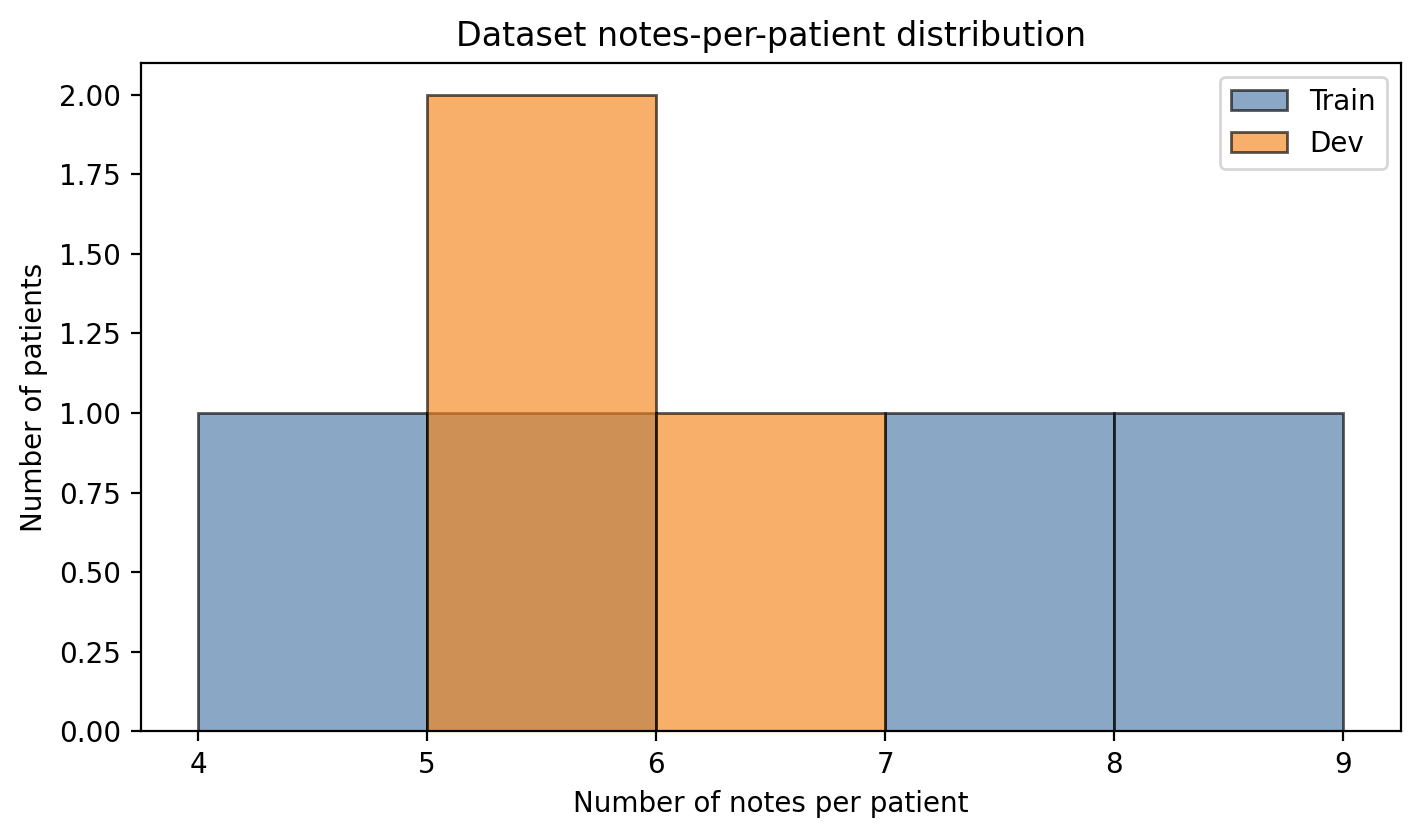
\includegraphics[width=\textwidth]{../assets/notes_per_patient_train_dev.png}
  \caption{Notes-per-patient distribution.}
\end{subfigure}
\hfill
\begin{subfigure}[b]{0.48\textwidth}
  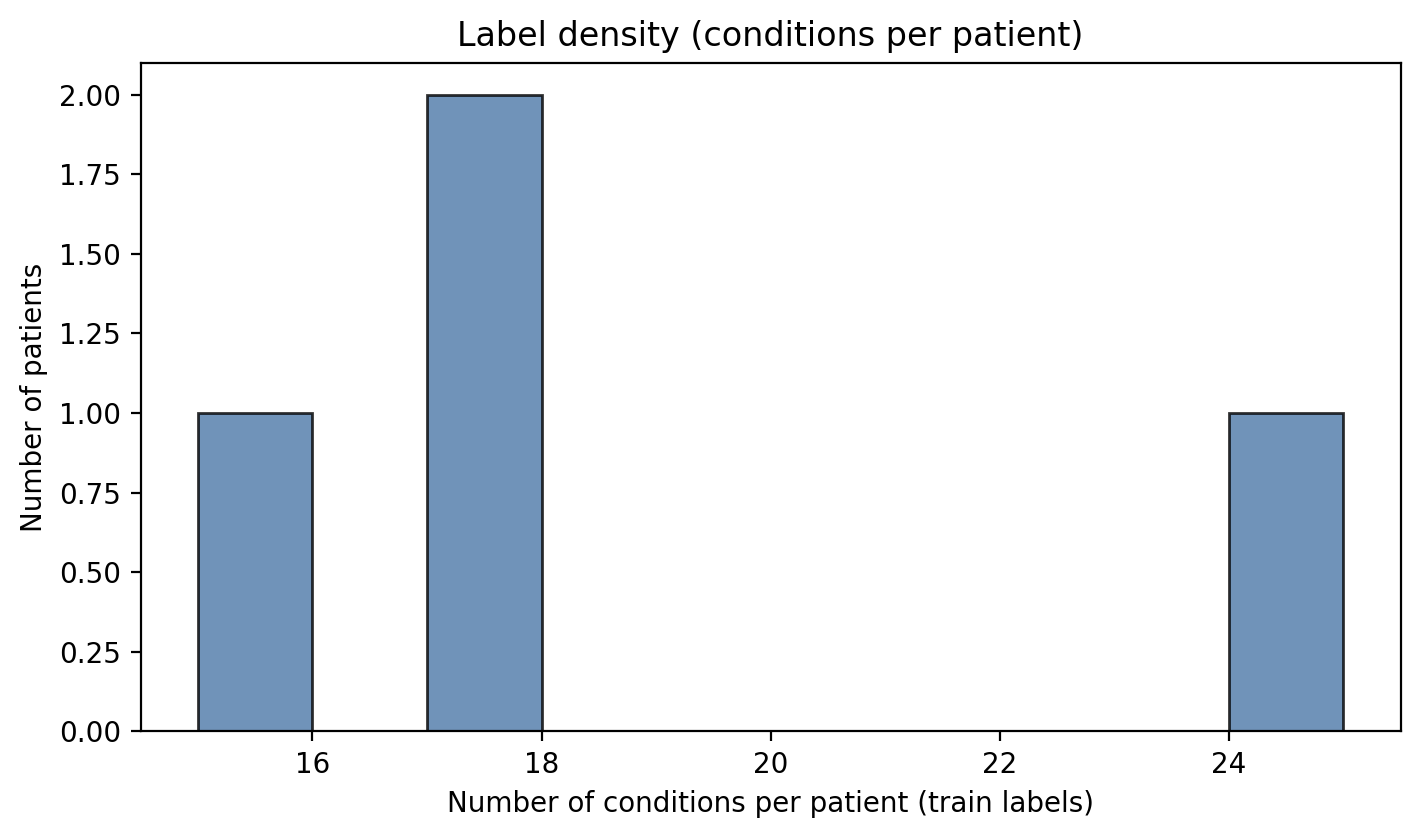
\includegraphics[width=\textwidth]{../assets/conditions_per_patient_train.png}
  \caption{Conditions per patient (training labels).}
\end{subfigure}
\caption{Dataset statistics: note and condition density.}
\end{figure}

\subsection{Label Analysis}

Training labels reveal important patterns for system design:

\begin{table}[H]
\centering
\caption{Training label statistics (across 73 conditions from 4 patients).}
\begin{tabular}{lc}
\toprule
\textbf{Statistic} & \textbf{Value} \\
\midrule
Total evidence entries & 356 \\
Avg evidence/condition & 4.9 \\
Evidence range & 1--14 per condition \\
Onset date coverage & 100\% (all have dates) \\
Conditions per patient & 15--24 \\
\bottomrule
\end{tabular}
\end{table}

\begin{figure}[H]
\centering
\begin{subfigure}[b]{0.48\textwidth}
  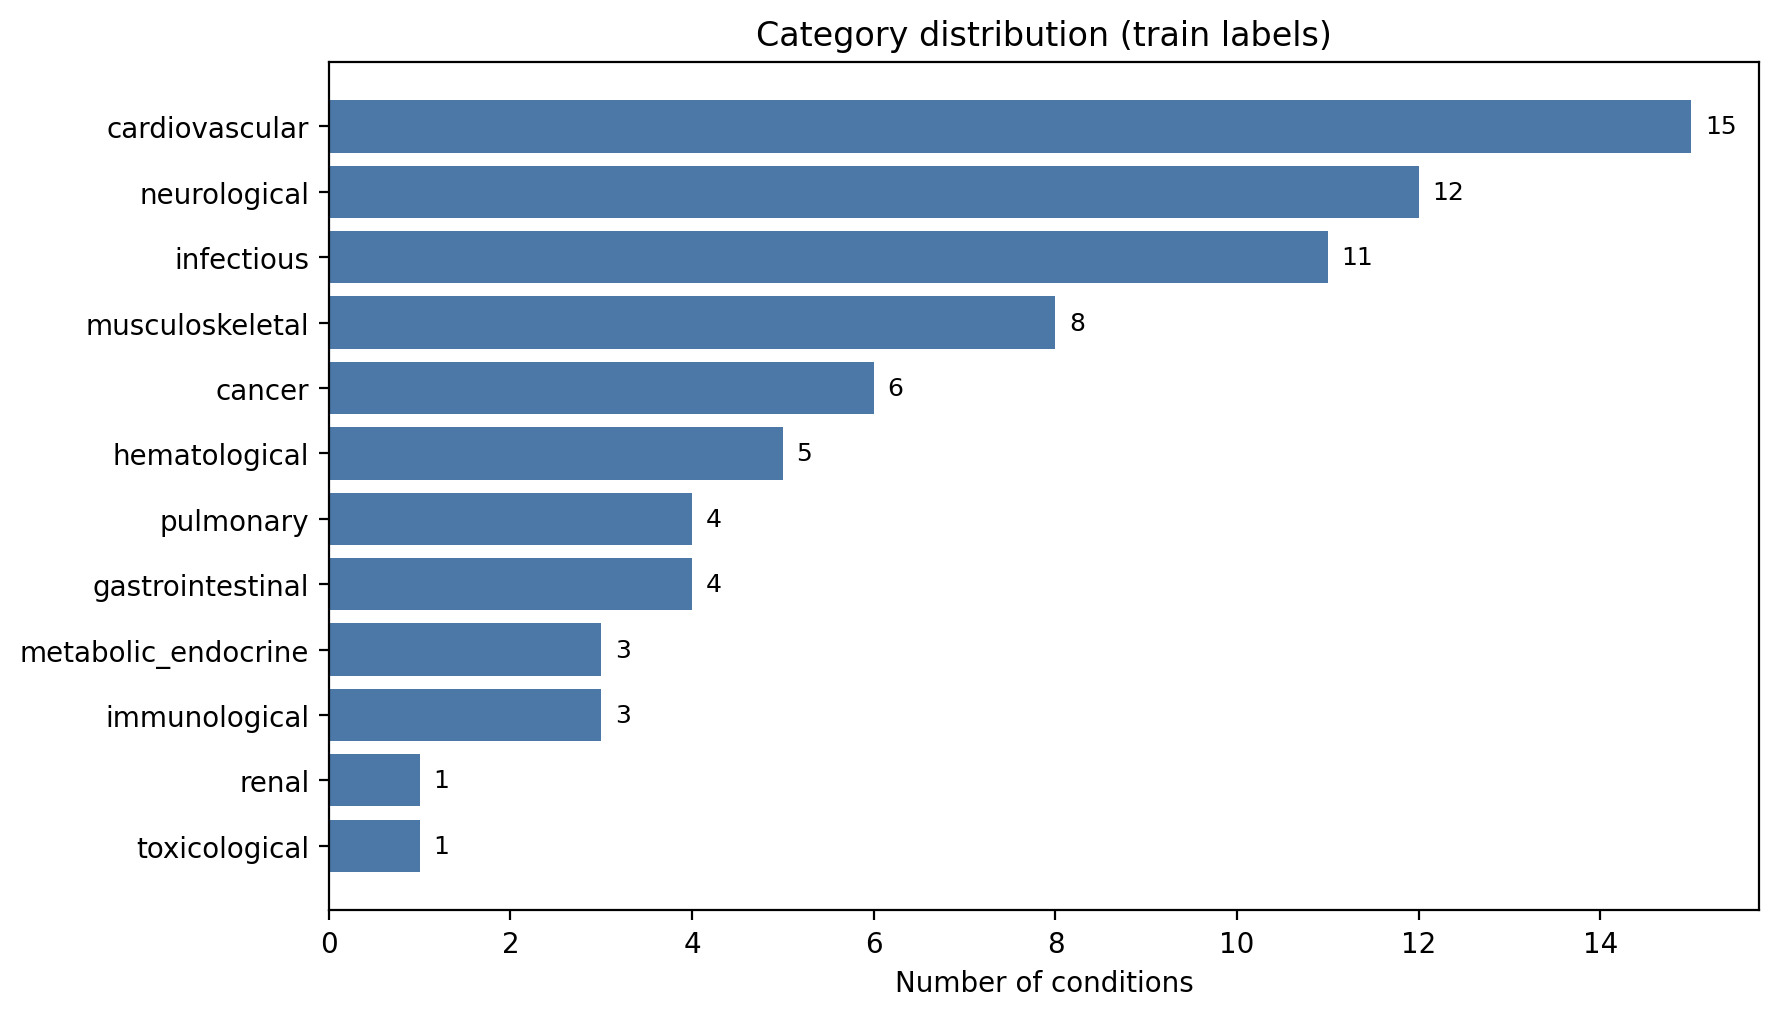
\includegraphics[width=\textwidth]{../assets/label_category_distribution_train.png}
  \caption{Category distribution.}
\end{subfigure}
\hfill
\begin{subfigure}[b]{0.48\textwidth}
  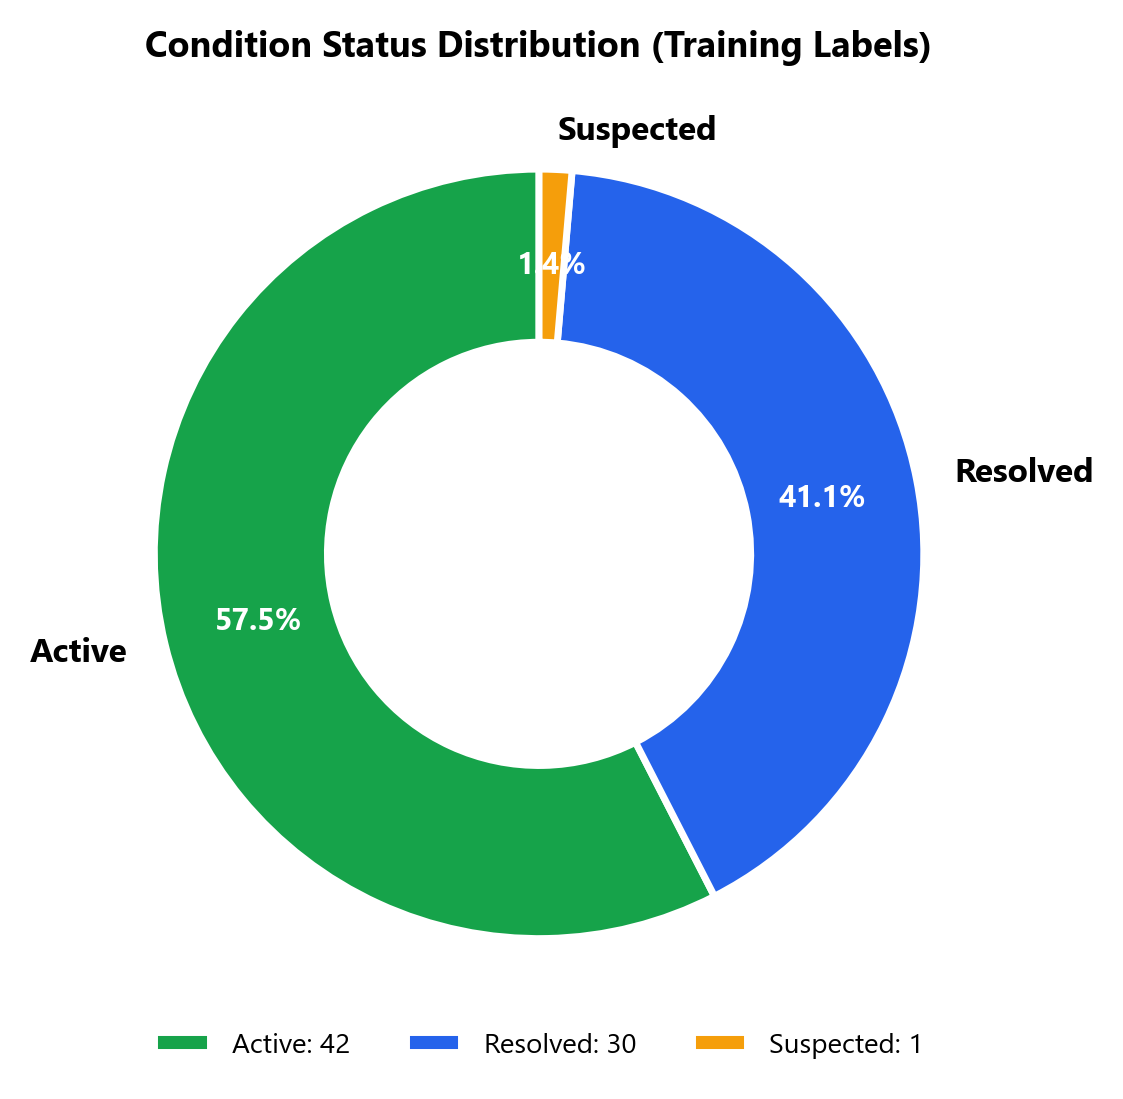
\includegraphics[width=\textwidth]{../assets/status_distribution_train.png}
  \caption{Status distribution.}
\end{subfigure}
\caption{Training label distributions by category and condition status.}
\end{figure}

\begin{figure}[H]
\centering
\begin{subfigure}[b]{0.48\textwidth}
  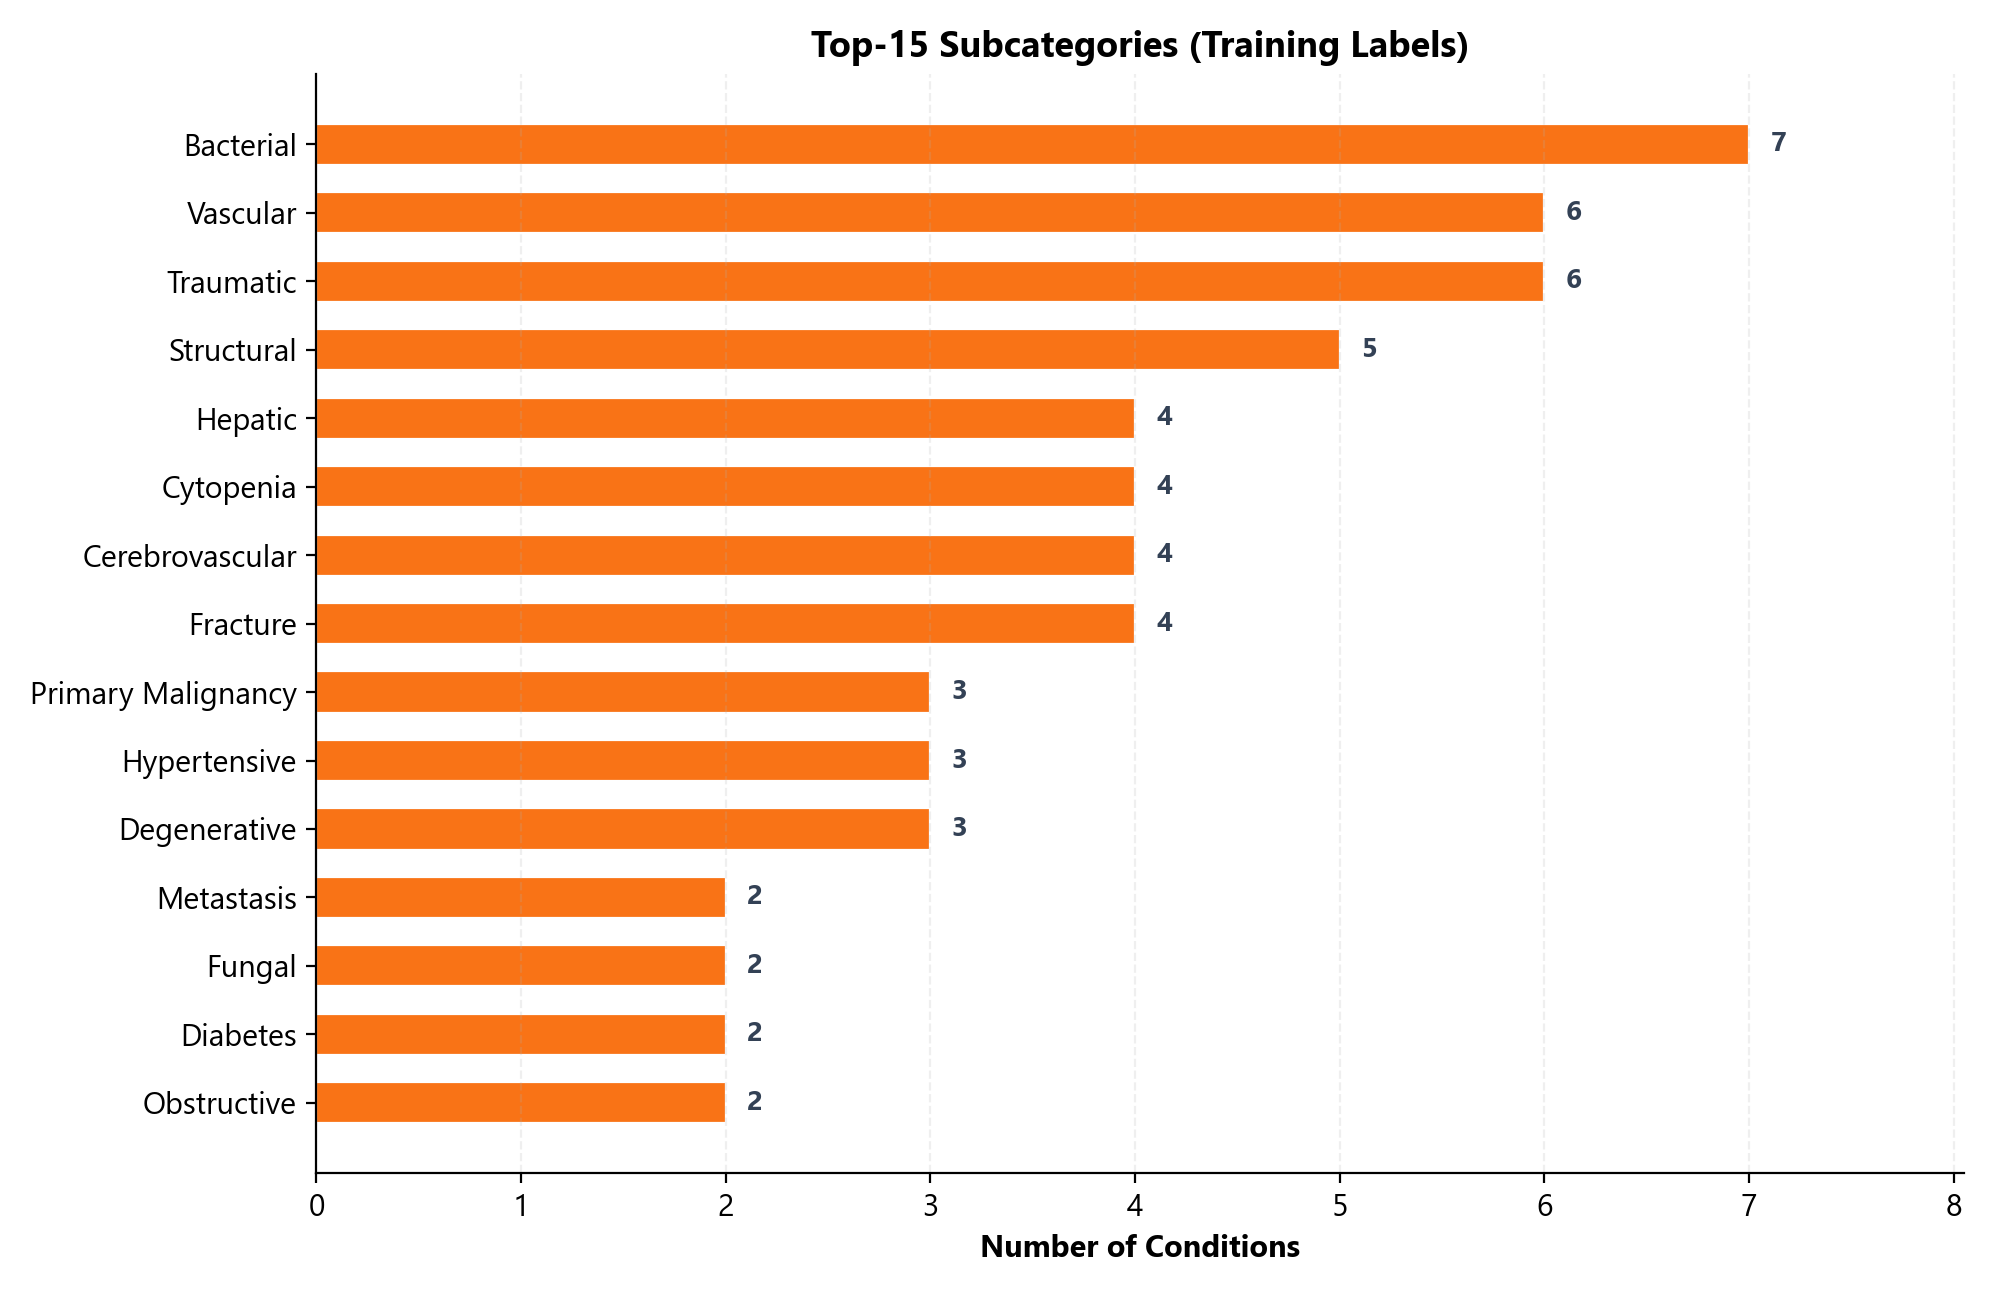
\includegraphics[width=\textwidth]{../assets/label_subcategory_top15_train.png}
  \caption{Top-15 subcategories.}
\end{subfigure}
\hfill
\begin{subfigure}[b]{0.48\textwidth}
  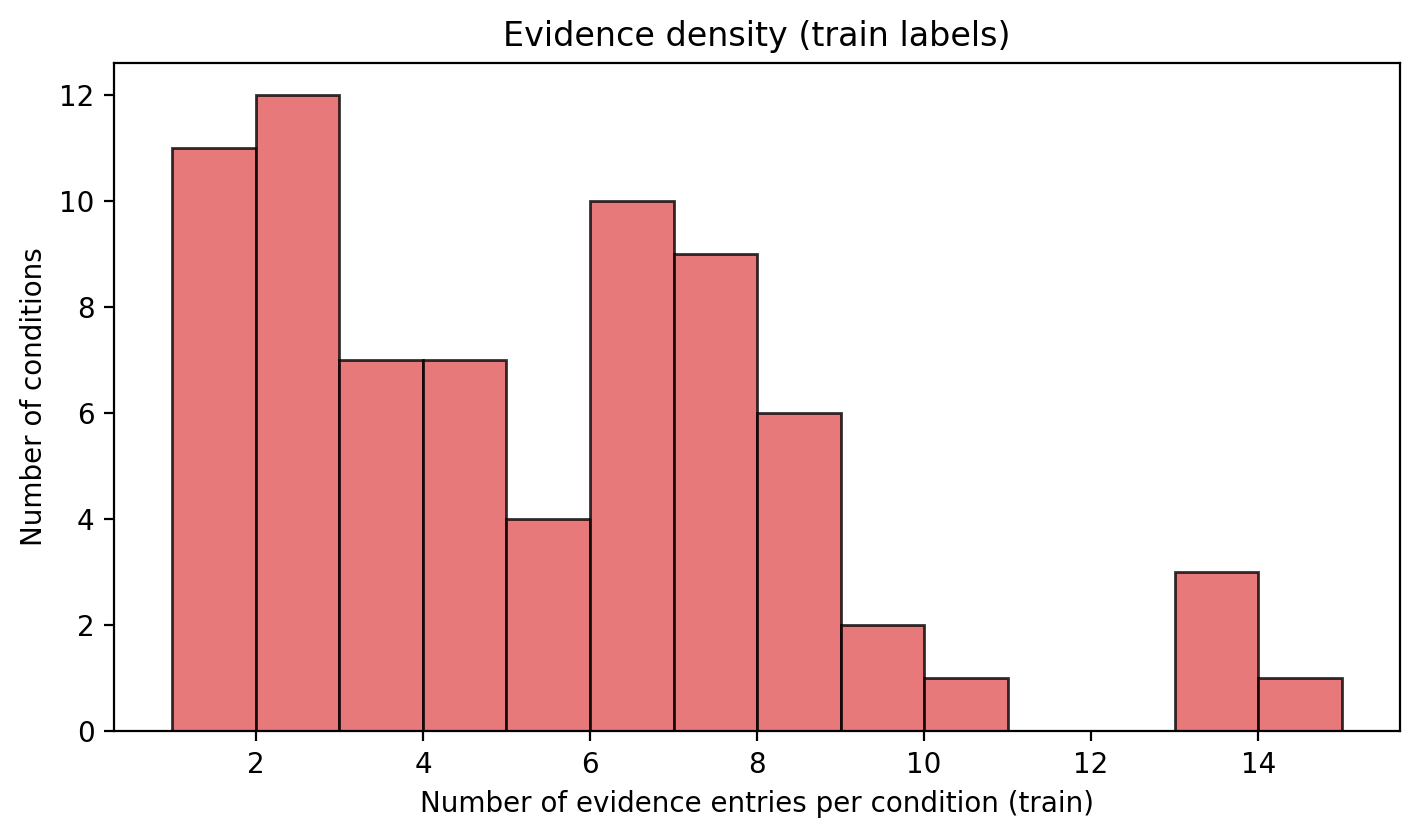
\includegraphics[width=\textwidth]{../assets/evidence_entries_histogram_train.png}
  \caption{Evidence entries per condition.}
\end{subfigure}
\caption{Subcategory frequency and evidence density analysis.}
\end{figure}

\subsection{Key Observations}

\begin{enumerate}[leftmargin=1.2em, itemsep=2pt]
  \item \textbf{Naming variance}: The same condition appears with different names across notes (e.g., ``Diabetes mellitus type II'' vs.\ ``Non-insulin-dependent diabetes mellitus type II'').
  \item \textbf{Multi-section extraction}: Conditions appear in structured sections (Diagnoses, Other Diagnoses, Medical History) AND in narrative text, imaging reports, and lab results.
  \item \textbf{Lab-derived conditions}: Abnormal lab values (e.g., Hemoglobin 8.2\,g/dL) imply clinical conditions (anemia) even when not explicitly named.
  \item \textbf{High condition density}: Average 18.2 conditions per patient requires handling large extraction volumes without truncation.
  \item \textbf{Temporal complexity}: Notes contain absolute, relative, and implicit dates requiring sophisticated resolution.
\end{enumerate}

% =====================================================================
\section{System Architecture}
% =====================================================================

The system implements a \textbf{three-stage pipeline} --- two LLM-driven passes followed by a deterministic hardening pass --- designed for maximum recall with strict schema compliance.

\begin{figure}[H]
\centering
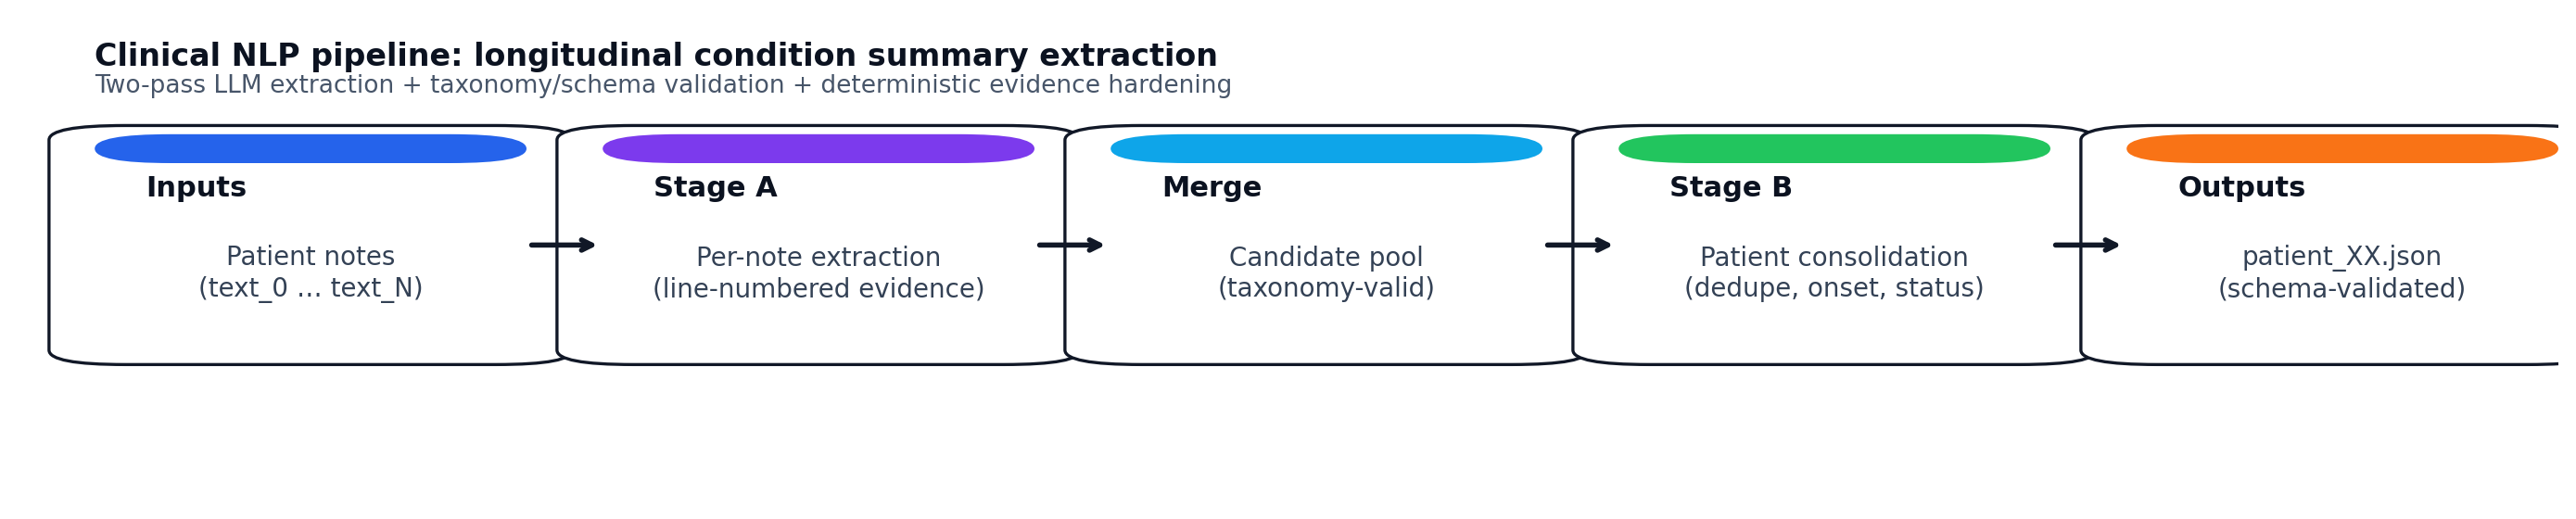
\includegraphics[width=0.98\linewidth]{../assets/pipeline.png}
\caption{End-to-end extraction pipeline: Data Ingestion $\rightarrow$ Per-Note Extraction $\rightarrow$ Patient Consolidation $\rightarrow$ Evidence Hardening $\rightarrow$ Validated Output.}
\label{fig:pipeline}
\end{figure}

\subsection{Stage A: Per-Note Extraction (Map Phase)}

Each note is processed independently through the LLM:

\begin{enumerate}[leftmargin=1.2em, itemsep=2pt]
  \item \textbf{Load \& index}: Read the note with 1-indexed line numbers for precise evidence tracking.
  \item \textbf{Rich system prompt} (\texttt{prompts.py}): Full taxonomy with descriptions and examples, status definitions with signal keywords, disambiguation rules verbatim from taxonomy, onset priority rules, and a curated few-shot example ($\sim$15K characters, $\sim$4K tokens).
  \item \textbf{LLM extraction}: JSON output via \texttt{response\_format: json\_object} (with automatic fallback for unsupported providers).
  \item \textbf{Evidence span coercion}: Verify each \texttt{evidence.span} is an exact substring of the referenced \texttt{line\_no}; fallback to full line text if paraphrased.
  \item \textbf{Fuzzy taxonomy recovery}: Near-miss keys recovered via \texttt{rapidfuzz} ($\geq$75\% category, $\geq$70\% subcategory), saving $\sim$5\% of conditions.
  \item \textbf{Pydantic validation}: Strict schema enforcement with \texttt{extra="ignore"} for resilience against bonus LLM fields.
\end{enumerate}

\subsection{Stage B: Patient-Level Consolidation (Reduce Phase)}

All per-note candidates are consolidated via a second LLM call:

\begin{table}[H]
\centering
\caption{Consolidation strategies for each condition attribute.}
\begin{tabular}{ll}
\toprule
\textbf{Attribute} & \textbf{Strategy} \\
\midrule
\textbf{Deduplication} & Fuzzy name matching ($\geq$88\%) within same taxonomy slot \\
\textbf{Status} & From chronologically latest note where condition appears \\
\textbf{Onset} & Earliest non-null date (stated date $>$ note date $>$ relative) \\
\textbf{Evidence} & Retain from every note where condition is mentioned \\
\textbf{Name} & Most specific/descriptive among merged candidates \\
\bottomrule
\end{tabular}
\end{table}

\begin{keyinsight}
If the consolidation LLM output fails Pydantic validation, the system automatically falls back to a \textbf{deterministic merge}: deduplicate by normalized name + taxonomy slot, earliest onset, latest status, union of evidence. This guarantees schema-valid output regardless of LLM behavior.
\end{keyinsight}

\subsection{Stage C: Evidence Hardening (Deterministic Post-Pass)}

A zero-cost deterministic pass after consolidation:

\begin{itemize}[leftmargin=1.2em, itemsep=2pt]
  \item Scans all note lines for fuzzy matches against each condition name (partial ratio $\geq$90 via \texttt{rapidfuzz}).
  \item Adds at most one evidence entry per missing note (exact line text as \texttt{span}).
  \item Deduplicates evidence by \texttt{(note\_id, line\_no)}.
  \item \textbf{Cost}: Zero additional LLM calls --- only string matching operations.
\end{itemize}

\begin{figure}[H]
\centering
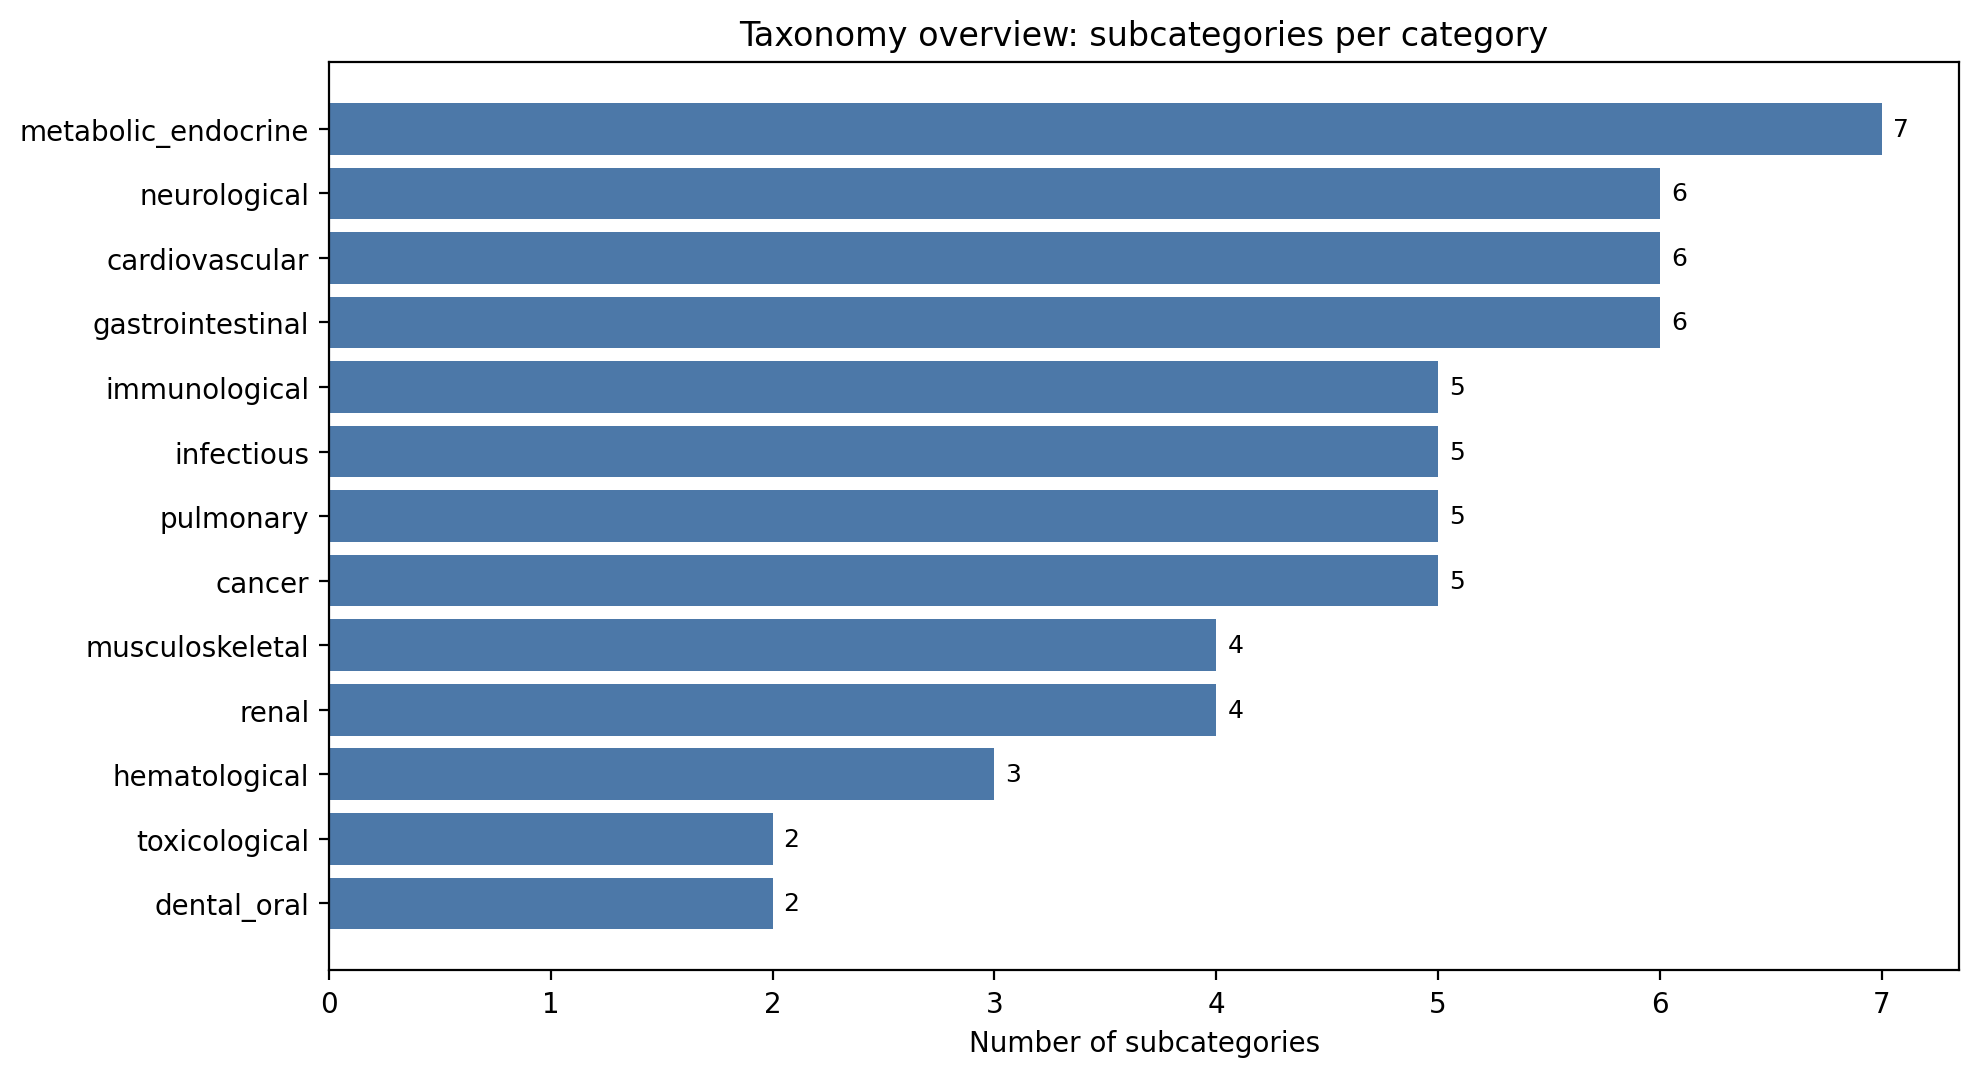
\includegraphics[width=0.98\linewidth]{../assets/taxonomy_overview.png}
\caption{Clinical taxonomy structure: 13 categories with 2--7 subcategories each.}
\end{figure}

% =====================================================================
\section{Design Decisions \& Rationale}
% =====================================================================

\begin{table}[H]
\centering
\caption{Key design decisions with rationale and impact.}
\small
\begin{tabularx}{\textwidth}{p{3.8cm}X}
\toprule
\textbf{Decision} & \textbf{Rationale} \\
\midrule
Full taxonomy in prompts ($\sim$15K chars) & LLM needs context on subcategory semantics (e.g., ``primary\_malignancy'' vs.\ ``metastasis'') to classify correctly. Keys-only leads to frequent misclassification. \\
\addlinespace
Disambiguation rules verbatim & Without rules, LLMs consistently miscategorize heart failure and diabetic complications. Verbatim inclusion ensures domain-specific logic. \\
\addlinespace
Few-shot example (8 conditions) & Grounds non-obvious behaviors: lab-derived conditions, procedure exclusion, multi-line evidence, edge-case taxonomy mapping. \\
\addlinespace
Fuzzy taxonomy recovery & LLMs output near-miss keys $\sim$5\% of the time. Recovery prevents direct recall penalty without introducing false positives. \\
\addlinespace
Evidence hardening & LLMs frequently omit evidence from notes where conditions are mentioned briefly. Deterministic post-pass catches these with zero additional cost. \\
\addlinespace
\texttt{max\_output\_tokens} = 4096 & Patient\_16 has 24 conditions --- full JSON exceeds 2048 tokens. Prevents truncation-induced invalid JSON. \\
\addlinespace
Disk caching (SHA-256) & Content-addressed cache enables fast iterative development. Prompts that change trigger fresh API calls automatically. \\
\addlinespace
Parallel per-note extraction & Notes within a patient are independent during Stage~A. \texttt{ThreadPoolExecutor} with \texttt{--concurrency\,4} provides 2--4$\times$ speedup. \\
\addlinespace
Robust JSON parsing & Multi-strategy extraction (direct $\rightarrow$ fenced block $\rightarrow$ brace-delimited) handles all observed LLM output formats. \\
\addlinespace
\texttt{response\_format} fallback & Automatically detects unsupported providers and retries with ``respond in JSON only'' system prompt suffix. \\
\bottomrule
\end{tabularx}
\end{table}

% =====================================================================
\section{Prompt Engineering}
% =====================================================================

\subsection{Per-Note System Prompt}

The system prompt for Stage~A follows a structured 9-section layout:

\begin{enumerate}[leftmargin=1.2em, itemsep=1pt]
  \item Role definition (``expert clinical information extraction system'')
  \item Full taxonomy with descriptions and examples
  \item Status value definitions with clinical signals
  \item Disambiguation rules (verbatim from taxonomy)
  \item Onset/date priority rules with format specifications
  \item 10 specific extraction guidelines
  \item Output format specification with JSON schema template
  \item Hard constraints (evidence exactness, taxonomy strictness)
  \item Few-shot example with key observations
\end{enumerate}

\subsection{Key Extraction Guidelines}

The prompt encodes 10 specific rules, including:

\begin{itemize}[leftmargin=1.2em, itemsep=1pt]
  \item Extract from ALL sections: Diagnoses, Medical History, imaging, labs, narrative
  \item Conditions in ``Medical History'' $\rightarrow$ \texttt{resolved} UNLESS chronic/ongoing (e.g., hypertension $\rightarrow$ \texttt{active})
  \item Lab abnormalities outside reference ranges $\rightarrow$ extract implied condition
  \item Do NOT extract symptoms alone (cough, fatigue) or surgical procedures
  \item One entry per distinct condition; separate entries per anatomical site
  \item Preserve site-specific qualifiers in condition names
\end{itemize}

\subsection{Consolidation Prompt}

Stage~B focuses on deduplication with synonym handling, chronological status resolution, onset priority across notes, and an explicit evidence completeness mandate: ``include evidence from ALL notes where mentioned.''

% =====================================================================
\section{Evaluation Framework}
% =====================================================================

The evaluation framework (\texttt{evaluate.py}, \texttt{train.py}) covers all six official scoring dimensions:

\begin{table}[H]
\centering
\caption{Evaluation metrics matching the official scoring criteria.}
\begin{tabular}{llp{7.5cm}}
\toprule
\textbf{Metric} & \textbf{Type} & \textbf{Description} \\
\midrule
Condition Precision & P/R/F1 & Fraction of predicted conditions correctly matched (category + subcategory + fuzzy name $\geq$88\%) \\
Condition Recall & P/R/F1 & Fraction of ground-truth conditions found \\
Condition F1 & P/R/F1 & Harmonic mean of precision and recall \\
Status Accuracy & Accuracy & \% of matched conditions with correct status (exact string match) \\
Onset Exact & Accuracy & \% with exact onset date match \\
Onset Partial & Accuracy & \% with at least correct year (via regex) \\
Evidence Recall & Fraction & GT evidence \texttt{note\_id}s covered per condition \\
Evidence Precision & Fraction & Relevant / total predicted evidence entries \\
\bottomrule
\end{tabular}
\end{table}

\begin{figure}[H]
\centering
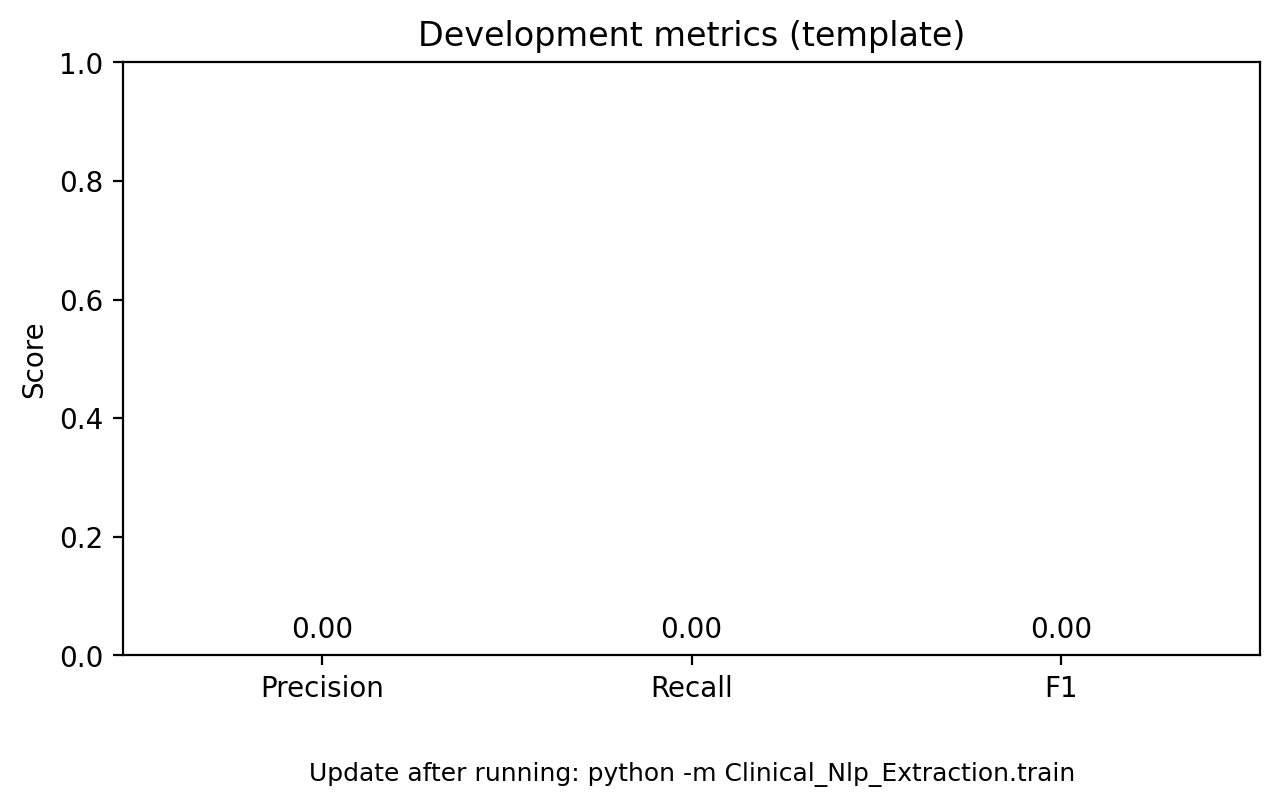
\includegraphics[width=0.72\linewidth]{../assets/metrics_plot.png}
\caption{Evaluation metrics dashboard template. Populate by running: \texttt{python -m Clinical\_Nlp\_Extraction.train --results-json results.json}}
\end{figure}

\noindent\textbf{Evaluation command:}
\begin{lstlisting}
python -m Clinical_Nlp_Extraction.train \
  --data-dir ./Data/train \
  --taxonomy-path ./Data/taxonomy.json \
  --results-json ./results.json --verbose
\end{lstlisting}

% =====================================================================
\section{Reproducibility, Speed, and Cost}
% =====================================================================

\begin{table}[H]
\centering
\caption{Reproducibility and performance characteristics.}
\begin{tabular}{lp{10cm}}
\toprule
\textbf{Feature} & \textbf{Implementation} \\
\midrule
Caching & SHA-256 hash of prompt content $\rightarrow$ disk cache; re-runs produce identical outputs with zero API calls \\
Determinism & Default temperature 0.0 \\
Token tracking & Cumulative prompt + completion + latency per call; summary at end of each run \\
Parallelism & \texttt{ThreadPoolExecutor} with configurable \texttt{--concurrency} (default: 4); 2--4$\times$ speedup \\
\bottomrule
\end{tabular}
\end{table}

\subsection{Cost Estimation}

\begin{table}[H]
\centering
\caption{Estimated token usage per patient (6 notes).}
\begin{tabular}{lrl}
\toprule
\textbf{Component} & \textbf{Tokens} & \textbf{Type} \\
\midrule
Stage A system prompts & $\sim$24K & Input ($\sim$4K $\times$ 6 notes) \\
Stage A note content & $\sim$9K & Input ($\sim$1.5K $\times$ 6 notes) \\
Stage A outputs & $\sim$12K & Output ($\sim$2K $\times$ 6 notes) \\
Stage B consolidation prompt & $\sim$8K & Input \\
Stage B output & $\sim$4K & Output \\
\midrule
\textbf{Total per patient} & $\sim$\textbf{57K} & \\
\bottomrule
\end{tabular}
\end{table}

% =====================================================================
\section{How to Run}
% =====================================================================

\subsection{Installation}
\begin{lstlisting}
pip install -r requirements.txt
\end{lstlisting}

\noindent\textbf{Dependencies:} \texttt{openai}$\geq$1.0.0, \texttt{tqdm}$\geq$4.60.0, \texttt{tenacity}$\geq$8.0.0, \texttt{pydantic}$\geq$2.6.0, \texttt{rapidfuzz}$\geq$3.6.0

\subsection{Environment Variables}
\begin{lstlisting}
export OPENAI_BASE_URL="https://api.openai.com/v1"
export OPENAI_API_KEY="sk-..."
export OPENAI_MODEL="gpt-4o"
\end{lstlisting}

\subsection{Inference (Primary Entrypoint)}
\begin{lstlisting}
python main.py \
  --data-dir ./Data/dev \
  --patient-list ./patients_dev.json \
  --output-dir ./output \
  --cache-dir ./.cache \
  --temperature 0 --concurrency 4
\end{lstlisting}

\subsection{Dry-Run (No API Calls)}
\begin{lstlisting}
python main.py --data-dir ./Data/dev \
  --patient-list ./patients_dev.json \
  --output-dir ./output_dry --dry-run
\end{lstlisting}

\subsection{Validate Outputs}
\begin{lstlisting}
python -m Clinical_Nlp_Extraction.validate_outputs \
  --output-dir ./output \
  --taxonomy-path ./Data/taxonomy.json
\end{lstlisting}

\subsection{CLI Arguments}

\begin{table}[H]
\centering
\caption{Complete CLI argument reference for \texttt{main.py}.}
\begin{tabular}{llp{7.5cm}}
\toprule
\textbf{Argument} & \textbf{Default} & \textbf{Description} \\
\midrule
\texttt{--data-dir} & \emph{required} & Path to data directory \\
\texttt{--patient-list} & \emph{required} & JSON list of patient IDs \\
\texttt{--output-dir} & \emph{required} & Output directory \\
\texttt{--taxonomy-path} & \texttt{Data/taxonomy.json} & Taxonomy definition \\
\texttt{--cache-dir} & \texttt{.cache} & LLM response cache \\
\texttt{--temperature} & 0.0 & LLM sampling temperature \\
\texttt{--max-output-tokens} & 4096 & Max tokens per LLM response \\
\texttt{--concurrency} & 4 & Parallel extraction threads \\
\texttt{--verbose} & off & Debug logging \\
\texttt{--dry-run} & off & Empty outputs, no LLM calls \\
\bottomrule
\end{tabular}
\end{table}

% =====================================================================
\section{Module Architecture}
% =====================================================================

\begin{table}[H]
\centering
\caption{Module responsibilities and key features.}
\small
\begin{tabularx}{\textwidth}{lX}
\toprule
\textbf{Module} & \textbf{Responsibility} \\
\midrule
\texttt{main.py} & CLI entrypoint: argument parsing, patient loop, dry-run mode, manifest generation \\
\texttt{data\_loader.py} & 1-indexed line loading, chronological note ordering, taxonomy/label parsing \\
\texttt{llm\_client.py} & OpenAI-compatible client with exponential backoff retry (4 attempts), \texttt{response\_format} fallback, robust JSON extraction, token/latency tracking \\
\texttt{model.py} & Client factory from environment variables \\
\texttt{prompts.py} & Prompt construction: full taxonomy, status/disambiguation/onset rules, few-shot example ($\sim$387 LOC) \\
\texttt{schemas.py} & Pydantic v2 models: \texttt{Condition}, \texttt{Evidence}, \texttt{PatientOutput}, \texttt{Taxonomy} \\
\texttt{extractor.py} & Two-pass extraction engine, evidence coercion \& hardening, fuzzy taxonomy recovery, deduplication, deterministic fallback ($\sim$440 LOC) \\
\texttt{inference.py} & Patient pipeline orchestrator (\texttt{ThreadPoolExecutor}) \\
\texttt{evaluate.py} & P/R/F1, status, onset (exact + partial), evidence recall \& precision \\
\texttt{train.py} & Training evaluation with per-patient scoring and macro-averaging \\
\texttt{validate\_outputs.py} & Schema + taxonomy validation for output files \\
\texttt{utils.py} & SHA-256 hashing, name normalization, markdown cleaning, JSON I/O \\
\bottomrule
\end{tabularx}
\end{table}

% =====================================================================
\section{What Worked / What Didn't}
% =====================================================================

\subsection{What Worked}

\begin{table}[H]
\centering
\caption{Effective techniques and their observed impact.}
\begin{tabularx}{\textwidth}{p{4cm}X}
\toprule
\textbf{Technique} & \textbf{Impact} \\
\midrule
Two-stage extraction & Reduces missed conditions by over-extracting per-note then consolidating \\
Full taxonomy in prompts & Substantially improves category/subcategory accuracy vs.\ keys-only \\
Disambiguation rules & Prevents systematic errors (e.g., diabetic nephropathy $\rightarrow$ renal) \\
Evidence hardening & Deterministically fills evidence gaps across notes at zero cost \\
Fuzzy taxonomy recovery & Saves $\sim$5\% of conditions otherwise dropped for key typos \\
Disk caching & Fast iterative development; identical prompts never re-call API \\
Robust JSON parsing & Handles fenced code blocks, markdown wrapping across models \\
Few-shot example & Grounds non-obvious extraction behaviors (labs, procedure exclusion) \\
Parallel extraction & 2--4$\times$ speedup for multi-note patients \\
\bottomrule
\end{tabularx}
\end{table}

\subsection{Limitations \& Risks}

\begin{table}[H]
\centering
\caption{Known limitations and mitigations.}
\begin{tabularx}{\textwidth}{p{4cm}X}
\toprule
\textbf{Limitation} & \textbf{Mitigation} \\
\midrule
LLM compliance variance & Different models follow instructions differently; prompts may need tuning for the evaluation model \\
Evidence hardening noise & Fuzzy matching can occasionally add noisy evidence; strict threshold ($\geq$90) and normalized matching mitigate this \\
Onset date extraction & Relative date conversion (``since mid-December'' $\rightarrow$ ``December 2016'') is heavily model-dependent \\
Token cost & Rich prompts ($\sim$4K tokens/call) increase usage; offset by caching and improved accuracy \\
Single few-shot & More diverse examples could improve generalization; limited by prompt length budget \\
\bottomrule
\end{tabularx}
\end{table}

% =====================================================================
\section{Conclusion}
% =====================================================================

We presented a production-grade clinical NLP pipeline that combines LLM-driven extraction with deterministic post-processing to achieve robust, schema-compliant condition summaries from longitudinal patient notes. The three-stage architecture (per-note extraction $\rightarrow$ patient consolidation $\rightarrow$ evidence hardening) ensures comprehensive coverage while the multiple layers of validation (Pydantic schemas, fuzzy taxonomy recovery, evidence coercion, deterministic fallback) provide resilience against LLM inconsistencies.

Key innovations include: (1)~a rich prompt design embedding the full taxonomy with disambiguation rules and few-shot examples; (2)~deterministic evidence hardening that strengthens recall at zero additional API cost; (3)~multi-strategy robustness mechanisms (fuzzy recovery, response format fallback, JSON extraction) ensuring cross-model portability.

The system is designed for easy deployment: a single \texttt{main.py} entrypoint with configurable CLI arguments, environment-variable-based API configuration, disk caching for cost efficiency, and comprehensive evaluation tooling.

\end{document}
